% Should be <2 pages

% **Problems**

% **Needs to contain**
% - Hardware Description on a more detailed level

% **Structure**

% - Hardware section
%     - Overview
%     - Decisions
% - Software section
%     - Overview
%     - Decisions

The work in this paper is divided up into two major areas; the hardware and the software implementations. The aim of this section is to give an overview of the implementation and the design decisions made for each area.

\section{Hardware Implementation}

% Overview
A similar paper conducted at KTH earlier this year served as the main baseline for how the hardware was to be setup.\cite{hospital} The main components are the microcontroller, the scale as well as the ADC (Analog-to-Digital Converter). Apart from this, an adequate power source is needed to provide energy to all components. 

% Decisions
\subsection{Scale}
The scale used for this paper is a Tedea Huntleigh - Model 1022. It is a small and simple model, and the specific device used in this paper had a maximum capacity of 50 kg.\cite{load-cell-data} In figure \ref{fig:wiring} we can see the labels of the four wires needed to hook up the load cell. The \textit{Input+} and \textit{Input-} signify the voltage input and ground. \cite{load-cell-spec} \textit{Output+} and \textit{Output-} will output a positive respectively a negative charge of about 1.5 voltage . During weighing, the internal resistance in the load cell will change ever so slightly, and the two outputs will have a small difference in the millivoltage range. This difference represents the weight measurement, and can be translated to a corresponding kg/lb value. In general, the more voltage the scale is supplied with, the greater this millivoltage range can be, which (in theory) means larger accuracy when weighing. Bear in mind that no two load cells are the same, and need to be calibrated to output the correct kg/lb value. Even though no calibrations were made to the load cell during this paper, an increase in the voltage provided to the load cell did correlate to an increased stability in the values produced. 

\begin{figure}[h]
	\centering
	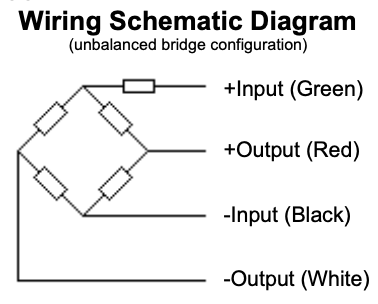
\includegraphics[width=0.3\textwidth]{load-cell-wiring.png}
	\caption{The wiring schematic for the load cell}
	\label{fig:wiring}
\end{figure}


\subsection{ADC}
To convert the millivoltage output from the load cell into a digital signal, an ADC is needed. The device used in this paper is an HX711, and apart from being a converter, it also serves as an amplifier for the load cell signal. We can see the front of the piece in figure \ref{fig:hx711}, and on the left side are the pinout where all the wires from the load cell should be connected. it is worth bearing in mind that the color coding of the wiring is not the same for all load cells, and the backside should be checked so that the connections follow the correct wiring schematic. 

It outputs data via two of its pins, the DAT and the CLK. The CLK pin will output 0 if it is ready to send data, and 1 if it is not ready. When it is ready, the DAT pin will send  a series of 0s and 1s that can be converted from binary to a decimal value, which will then represent the output of the load scale.\cite{hx711-datasheet} Multiple code libraries have been written to handle this for the user, and which only require a specification of which pins are being used by CLK and DAT respectively. For this paper, a library written for micropython was used.\cite{hx711-lopy}

\begin{figure}[h]
	\centering
	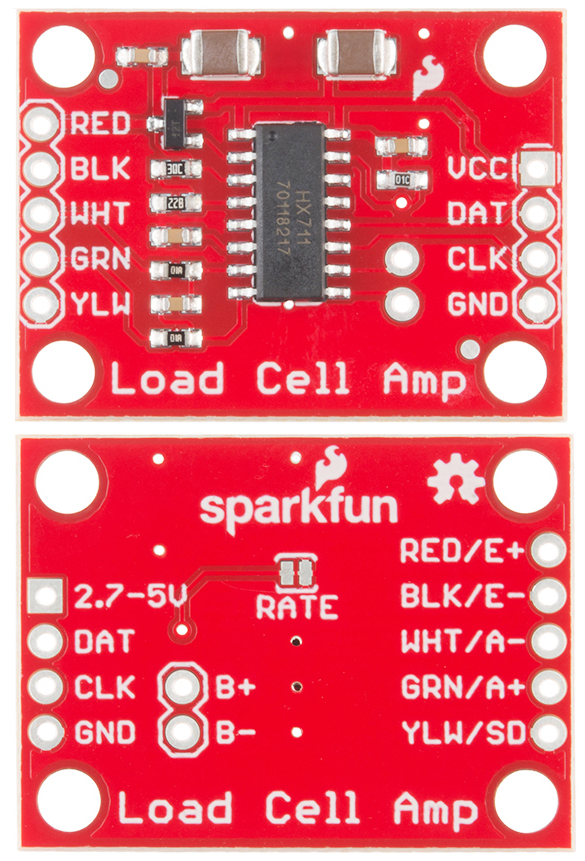
\includegraphics[width=0.3\textwidth]{hx711.png}
	\caption{The front and back of the HX711}
	\label{fig:hx711}
\end{figure}


\subsection{Microcontroller}
The microcontroller used for this paper was the FiPy development board from PyCom. It boasts a wide range of capabilities when it comes to communication protocols, NB-IoT being one of the five available.\cite{fipy-docs} With the supplied expansion board, connections via pinout is possible. It runs on micropython, which is an implementation of Python 3 optimized to run on microcontrollers.\cite{micropython}

%TODO: Add picture of FiPy and its expansion board

\subsection{Power Source}
In the early stages of the project, the hardware was powered via USB cable from a computer. Since the USB was of type micro, the voltage output was 5V. The benefit of this setup was a simple wiring schema where each component powered the next in line. The drawback was that the FiPy could only supply the ADC with 3V, which in turn affected the ADC's ability to read data from the load cell. During testing, the output rate of the raw data would be infrequent and erratic, sometimes taking several seconds to produce a single value. The values themselves did not correspond to increases and decreases in force being applied to the load cell, and would seemingly spike and crash at random. These problems were largely in part due to insufficient voltage being supplied to the ADC and load cell as later setups would reveal.
%TODO: Add schematic of this wiring

To remedy this, an approach using two different power sources was tried, where the ADC was powered by a wall outlet at a higher voltage, while the FiPy kept the USB. This resulted in electrical interference throughout the system, because of two different grounds being present in the circuit. The output rate of the data values had improved to a bit more stable rhythm than before, and the raw data values were a bit more responsive to the force applied to the load cell. 
%TODO: Add schematic of this wiring

The best setup that was tested involved an Otii battery toolbox, which is an advanced piece of hardware used to profile and emulate batteries.\cite{otii-web} With this piece of equipment, a common ground was provided to all components, as well as adequate voltage. It was capable of supplying 5V to both the FiPy and the ADC at the same time, which in turn enabled stable output of data values. When force was applied to the load cell, the data values responded accordingly with an increase or decrease in value. Due to time constraints and hardware availability, the setup could not be used for real network transmissions of the load cell data.
%TODO: Add schematic of this wiring

All data values produced by the load cell and ADC during these tests were raw values, as a calibration for kg/lb values for our intents and purposes would not bring any significant enhancements to the project.

\subsection{Wiring}
\begin{figure}[h]
	\centering
	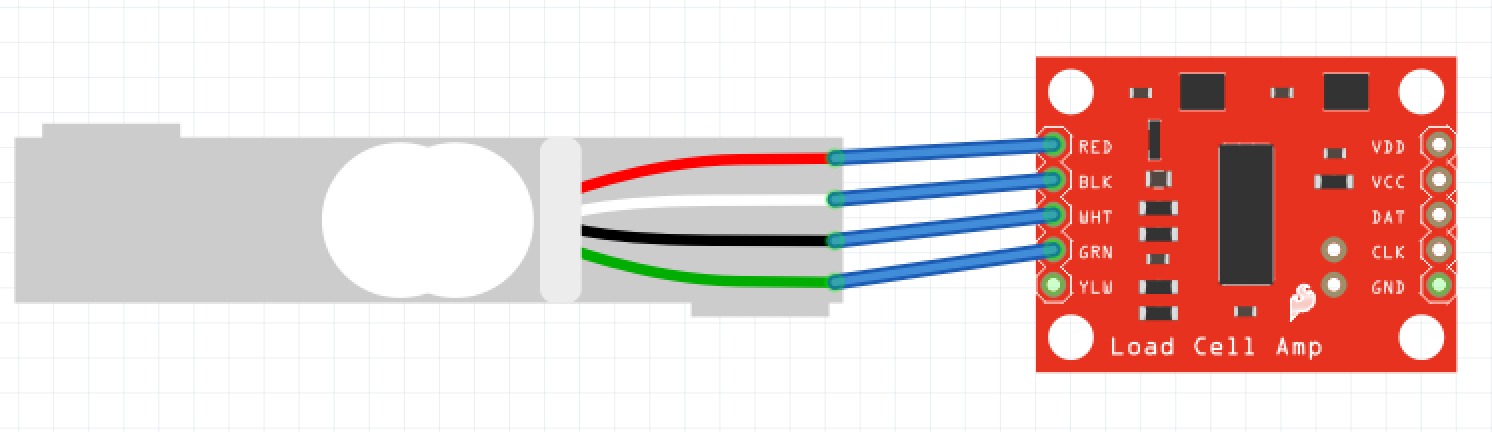
\includegraphics[width=0.6\textwidth]{load-cell_hx711.png}
	\caption{The load cell wired to the ADC}
	\label{fig:load-cell_hx711}
\end{figure}

\subsection{Failures}
During the first half of the project a faulty load cell was being used, which resulted in major delays of the hardware implementation. During the later half of the project no adequate solution to the problems with the power source could be devised in time for the practical testing of the hardware. Despite this, a short-lived setup with the Otii battery toolbox enabled a fairly functional load cell that could output tangible data values.



\section{Software Implementation}
The FiPy code runs on MicroPython, an implementation of Python 3 optimized for microcontrollers. MicroPython only executes two files on its system's root folder, the \lstinline{boot.py} and the \lstinline{main.py} files. Any remaining code must be placed in the \lstinline{/lib/} folder. The \lstinline{boot.py} runs first, and is intended to contain low-level code that is meant to configure the hardware. The \lstinline{main.py} file contains the main program loop, and imports auxiliary files from the \lstinline{/lib/} folder.
The two files used in the \lstinline{/lib/} folder are \lstinline{reader.py} and \lstinline{error_tracker.py}. A test file has been written for each module, to ensure that the software did not regress during development. All python classes and their respective tests can be found in the appendix. 

\subsection{reader.py}
The \lstinline{reader.py} file contains the \lstinline{Reader} class, which is responsible for processing the data polled from the load cell and passing it on to being transmitted. To instantiate a functional \lstinline{reader} object, it needs to be passed a poller function as well as a transmitter function. The purpose of having these functions passed to the instance of the class instead of being hardcoded into the class is to follow the separation of concern design principle.\cite{sep-concern} The poller function should accept no argument and is expected to return the current data value produced by the load cell when called. The transmitter function in turn should accept the data value to be transmitted.
%TODO: Add a more formal definition of what interface the functions should follow

The main method of the \lstinline{reader} instance is the \lstinline{run()} method. When called, the \lstinline{run()} method performs a cycle consisting of data polling, a check for false values, adjustment of the polling rate as well as a possible transmission. 

\subsubsection{Error Check}
The polled data value is subsequently checked for validity in the form of out-of-bounds values or extreme delta changes. A separate class called \lstinline{Error_tracker} monitors the interval and frequency of these occurrences, and the purpose of the class is to raise an exception when the error rate is deemed too high, and some form of remedial action needs to be taken. The internal workings of the \lstinline{Error_tracker} will be explained in a separate section.

\subsubsection{Adjustment of polling rate}
If the value is deemed valid, it is added to a FIFO (First-in, First-out) buffer of the most recent values. The contents of the buffer are then summed into a total delta value, which is used to adjust the polling rate. If the total delta surpasses a pre-defined threshold, the polling rate is increased, whereas if it is lower it might be maintained or decreased. When we say total delta value, we mean the delta values between two points, added to the delta of the next two points, as such:

$$\sum_{n=0}^{10} x_n - x_{n+1}$$


\subsection{error\_tracker.py}
The purpose of the Error\_tracker class is to keep track of the error occurrence and frequency. The intended usage is to instantiate an instance of the class, and call the \lstinline{error_occurred()} method when an invalid read has occurred. This method increases an internal counter, which will then raise an exception if it passes a pre-defined threshold.

\subsubsection{The Grace Period}
When invalid reads occur due to some temporary circumstance, it might not be beneficial to count all errors within a given timeframe towards raising an exception. We are not interested in sending an alert when short periods of errors occur, instead, it is at the long-lasting periods of polling errors an exception should be raised. To account for these short bursts, we use a \lstinline{GRACE_PERIOD} constant. This constant is used for the time window (in seconds) after the \lstinline{error_occurred()} method has been called, during which sequential calls  will not count toward the exception threshold.

\subsubsection{The Cooldown Period}
We do not want errors to rack up towards an exception over a longer period of time, so it would make sense to reset or decrease the internal error counter after a while. To enable this, a cooldown period is started after the grace period, during which any calls to to the \lstinline{error_occurred()} method will interrupt the cooldown period, and a new grace period will ensue. However, if the cooldown period ends without any calls being made to the \lstinline{error_occurred} method, the internal error counter will decrease by one. This way of self-regulation ensures that only a long-lasting and consistent frequency of errors raise an exception.


\subsection{Data Transmissions}
Data transmission tests were done separately from the load cell using dummy data. Pycom, the parent company behind the microcontroller used in this project also operate a cloud-based device management platform. \cite{pybytes-website} Via the pybytes platform, configuration of the network settings of the device can be managed via a firmware updater. 
In figure \ref{fig:wifi_longterm} and figure \ref{fig:wifi_raw_values} we can see data being transmitted via Wifi on a home network. The data is then displayed via graphs on the pybytes platform.

\begin{figure}[H]
\centering
	\begin{subfigure}[b]{0.3\textwidth}
    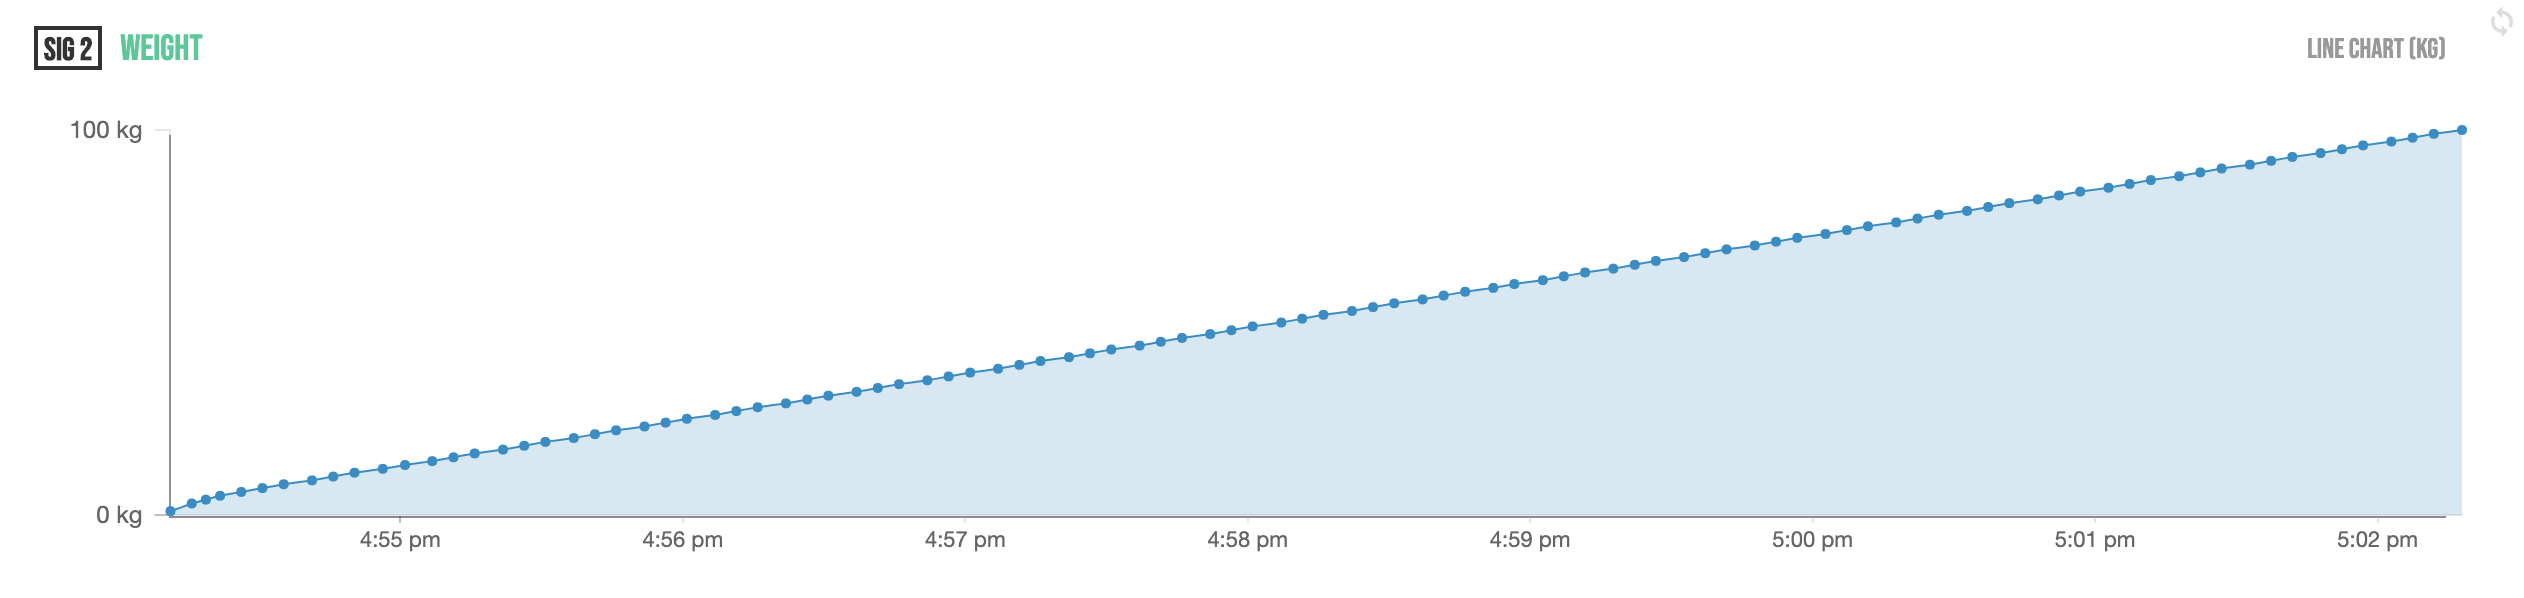
\includegraphics[width=\textwidth]{wifi_longterm.png}
    \caption{Data transmitted via Wifi}
    \label{fig:wifi_longterm}
	\end{subfigure}
	%
	\begin{subfigure}[b]{0.3\textwidth}
    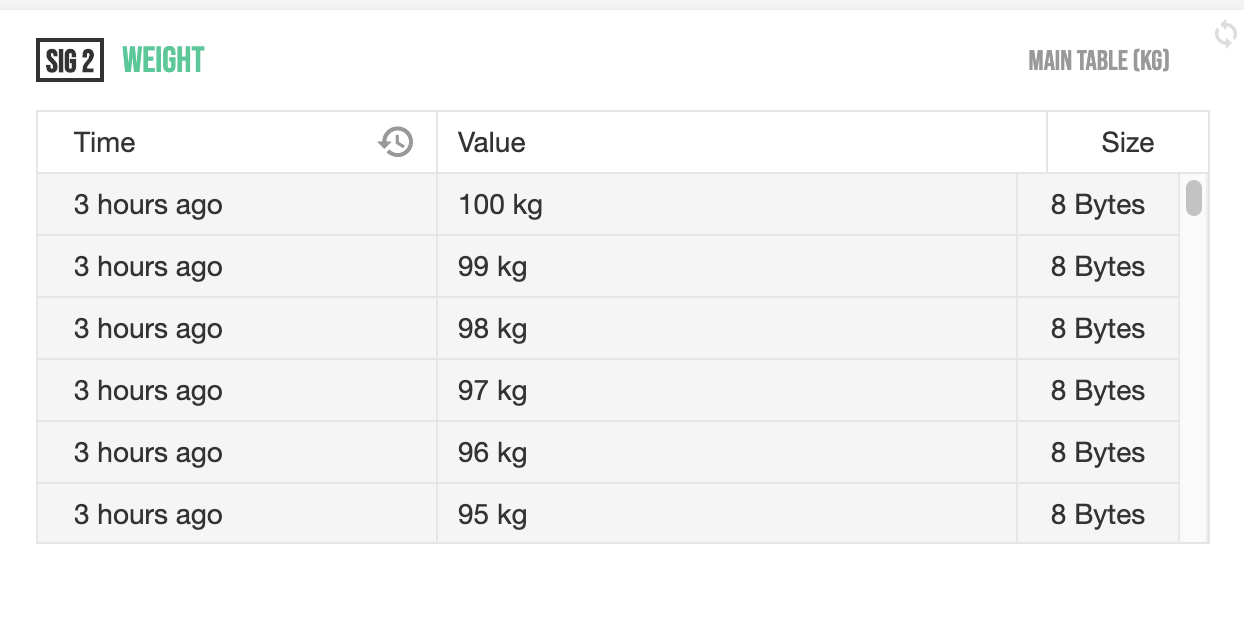
\includegraphics[width=\textwidth]{wifi_raw_values.png}
    \caption{}
    \label{fig:wifi_raw_values}
	\end{subfigure}
\end{figure}

Due to time limitations in the project, no actual tests of the transmission of the data via NB-IoT was made 